\documentclass{article}
\usepackage{graphicx} % Required for inserting images
\usepackage{acl2018}
\usepackage{float}
\usepackage[utf8]{inputenc} % allow utf-8 input
\usepackage[T1]{fontenc}    % use 8-bit T1 fonts
\usepackage{hyperref}       % hyperlinks
\usepackage{url}            % simple URL typesetting
\usepackage{booktabs}       % professional-quality tables
\usepackage{amsfonts}       % blackboard math symbols
\usepackage{nicefrac}       % compact symbols for 1/2, etc.
\usepackage{microtype}      % microtypography
\usepackage{xcolor}         % colors
\usepackage{siunitx}        % units
\sisetup{list-units = single}

\title{NLP Final Project Report: Sports Fans Sentiment Analysis}

\author{
  \begin{tabular}{c}
    Jianfeng Ke \\
    02031747
  \end{tabular}
  \begin{tabular}{c}
    Sameed Khan \\
    01987789
  \end{tabular}
  \begin{tabular}{c}
    Daheng Kuang \\
    01891533
  \end{tabular}
  \begin{tabular}{c}
    Sean Lynch \\
    01858462
  \end{tabular}
  \begin{tabular}{c}
    Anveshak Rathore \\
    02036112
  \end{tabular}
}


\begin{document}

\maketitle

\section*{Abstract}
The project looks at the sentiments of sports fans in different contexts. Going with the assumption that different fans respond differently to their sports team's results, the project aims to quantify if and when these fans respond differently. Using a state-of-the-art model, GoEmotions \cite{demszky-etal-2020-goemotions}, the project quantifies the difference in sentiments of fans from losing, winning, and other teams in 4 different contexts: the favorite or the underdog winning either a one-sided or close game. The research explores a previously untapped context of sports fan responses to specific external events. This allows us to see how different psychological responses are manifested in online language over time. Researchers would benefit by being able to delineate the emotions that different groups have at different times, and practitioners would know better when to target which specific groups of people.

\section{Introduction}

Fans of sports teams are often known to exhibit strong emotions while supporting teams. These emotions tend to be expressed and amplified even more on social media, which is the context of our project as well. This project's primary motive is to classify sports team fans' sentiments - before, during, and after the matches. The project looks at matches with two different types of results: the underdogs winning or the favorites winning. Our primary result shows the prevalence of two very contrasting emotions: annoyance and admiration. Beyond the initial classification measure, we also try another prediction task - predicting the result from the comments, and a second classification task: classifying sentiments of users over time, beyond just their responses to match events. The work is important for multiple reasons. Firstly, it offers interesting data points for the marketers to use for their targeting campaigns - targeting to annoyed potential consumers is very different from targeting potential consumers in the state of admiration. Secondly, it provides researchers with more insights into the mental states of online contributors split across an external event with known outcomes. Thirdly, it provides an understanding of how these mental states are manifested in online language over time.

\section{Related Works}

In the field of grief responses, we see that people react to losses in 5 stages: Denial and Isolation, Anger, Bargaining, Depression, and Acceptance. We can use these studies \cite{Mughal2023-rg} to see if sports fans fit in the same model and see how the emotions that we gather using Go-Emotions compare to the different stages of grief reaction.

There have been other models - for example, the Go-Emotion database, from software engineers and researchers at Amazon, Google Research, and Stanford. In the paper, they found that certain emotions were easier to model than others using the Reddit dataset\cite{demszky-etal-2020-goemotions}. This also provides us with a recently validated model for emotions using the same context (Reddit) and published at a top-tier conference after peer review, ACL 2020.

Reddit data itself has found use in similar studies. One such study uses text from nine-thousand users in order to classify them using Myers-Briggs personality type indicators\cite{gjurkovic-snajder-2018-Reddit}. Another uses Reddit-sourced text to train a model to detect offensive language within text\cite{hada-etal-2021-ruddit}. A comparison of emotional distributions can be seen in a study that used Reddit to find suitable users who resigned from their jobs and compared their comments before and after that date\cite{ireland-etal-2023-sadness}. By utilizing Reddit's API, we should no doubt be able to find sufficient data within our specified forums for any and all classifications of outcomes in sports games.

There has also been some limited work on sports fans' sentiments. A recent study \cite{iot1020014} looked at the sentiment of fan posts at the 2014 Soccer World Cup. However, they only used Naive Bayers, SVM, and other similar approaches. The authors also did not categorize the different types of events: wins and losses, that could specifically alter the emotions of the fans. 
\section{Method, Data and Results}

The method for the project comprised three different steps:
\begin{enumerate}
    \item Data Collection and Preprocessing
    \item Classification
    \item Analysis
\end{enumerate}

\subsection{Data Collection and Pre-processing}
The project required two different forms of data: match details and user comments. The match details were required to categorize the match into one of four categories: 
\begin{enumerate}
    \item Favorite wins a close match
    \item Underdog wins a close match
    \item Favorite wins a one-sided match
    \item Underdog wins a one-sided match
    
\end{enumerate}
The favorite and underdog were decided based on betting odds available across the websites. There was rarely any difference between different platforms in terms of who was considered the favorite, so the average odds from Wikipedia were taken. 
The second decision was on the definition of a "close" match compared to a "one-sided" match. Conversations with fans of the two sports we shortlisted (American football and soccer) provided a general idea that we felt was good enough: a game with less than a \textbf{10-point difference (American football)} or a \textbf{2-goal difference (soccer)} was considered a close game. Everything else was not.
Given the scope of the project, Reddit was the primary source used for the user comments' data. There were multiple reasons for this. Firstly, Reddit's structure of subreddits allows concentrated conversations to happen on a specific topic. Targeting r/nfl and r/soccer allowed us to look at the relevant discussions around these topics. Specifically within these categories of discussions, the focus was on match data. Reddit's sports subreddits often follow a method relying on Match Threads (and often pre-match and post-match threads) that provide a singular platform for all discussion relevant to the match. To ensure adequate representation for all 4 categories mentioned above, we ended up gathering Reddit threads for 24 matches across NFL and soccer, resulting in data for 10 SuperBowls and 1 regular season game for NFL, and 8 finals, and 3 other knockout matches from the UEFA Champions League in soccer.
From these match threads, the three important things gathered through the Reddit API were comment content, poster flair, and upvotes. Poster flair was significantly important because it showed the team supported by the commenter. This is also why a lot of the data had to be scraped by the team, and we couldn't rely on existing databases that did not have the comment flair. To provide some context, a sample comment with a commenter flair is shown below.
\begin{figure}[h]
    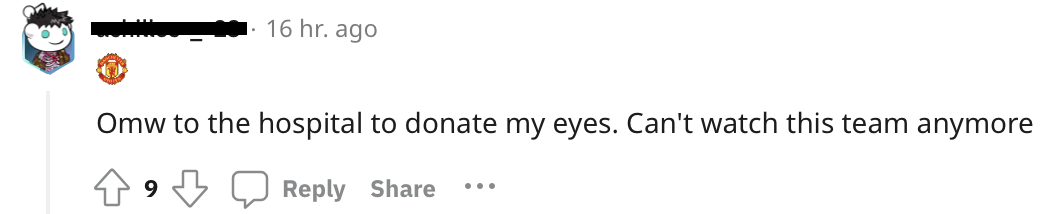
\includegraphics[width=\linewidth]{Comment.png}
    \caption{Sample Reddit comment with team flair}
\end{figure}


\subsection{Classification}
The classification of sentiments relied on two things: comment text from the matches specified above, and the Go-Emotions model. Given that the model was trained for sentiment classification on Reddit data, we did not need to further train or fine-tune the data. Go Emotion's model provides the probability for the following 28 emotions, which we predicted for 31,000+ comments.
\begin{figure}[h]
    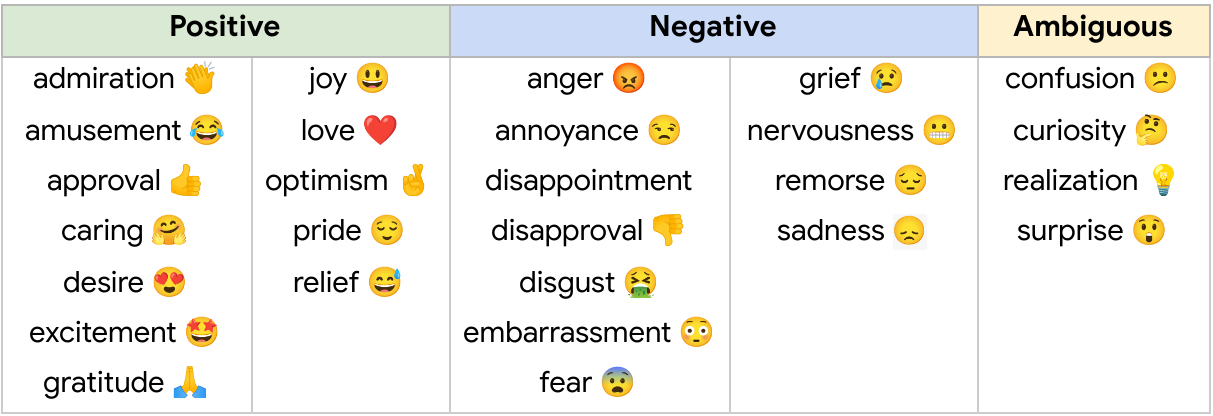
\includegraphics[width=8cm]{GoEmotions.png}
    \caption{Corpus of emotions in the GoEmotions model}
\end{figure}

\subsection{Analysis}
We show the final results by visualization and comparison between the emotion frequencies of different categories or groups. For example, we investigate how football fans react differently from soccer fans in general, how emotions in the population differ for matches in 4 different categories, and how people react differently when the match is in different phases.

\begin{figure}[h]
    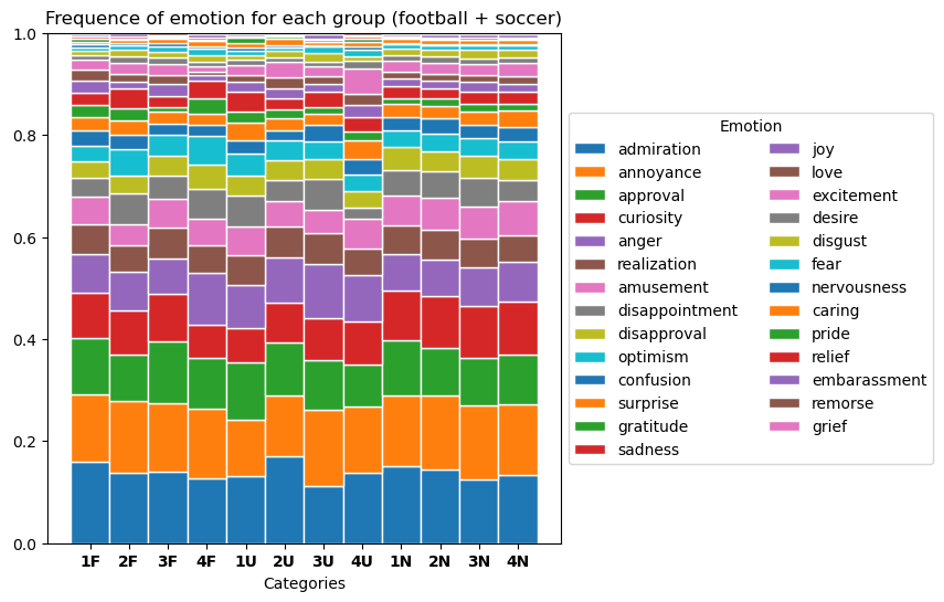
\includegraphics[width=8cm]{StackedFrequency.png}
    \caption{Stacked frequency plot for emotions for different types of matches and different group of people}
\end{figure}

Figure 3 shows the Stacked frequency of emotions of 3 types of viewers in 4 categories of matches. "F" stands for favored team supporters, "U" stands for underdog team supporters, and "N" stands for other neutral viewers. The definitions of 4 categories of matches are mentioned in section 3.1. In general, admiration, annoyance, and approval are the top 3 emotions with the highest frequencies. We noticed something interesting from the distribution plot, such as, admiration appears the most in the underdog team supporters when the underdog team wins a close match, and excitement appears the most when the underdog team wins a one-sided match.

\begin{figure}[h]
    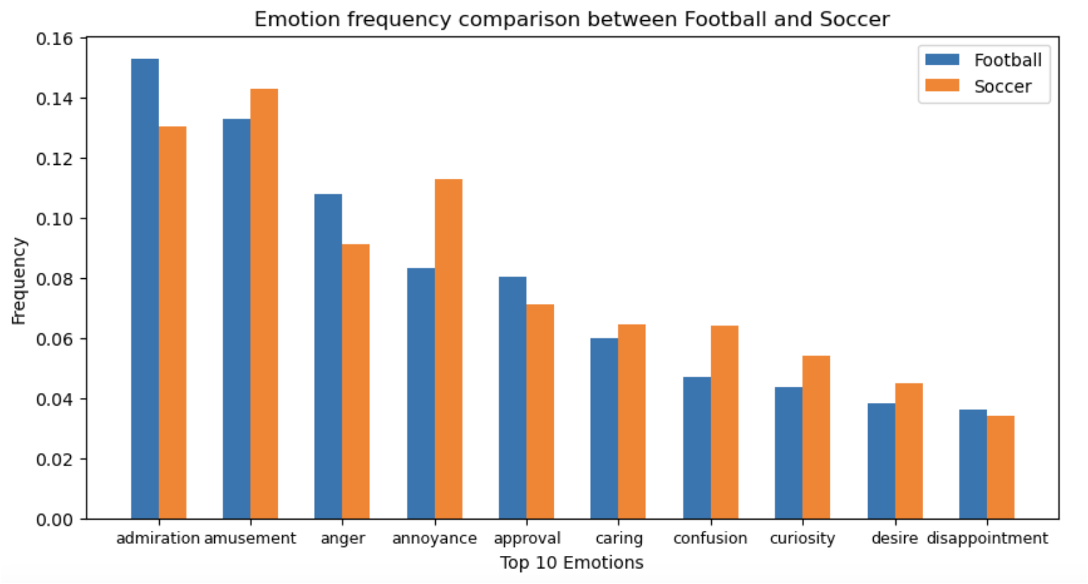
\includegraphics[width=8cm]{SportsComparision.png}
    \caption{Top 10 emotion frequency comparison between football and soccer}
\end{figure}

Figure 4 shows the emotion frequency comparison between football and soccer for the 10 emotions with the highest frequency. Admiration and anger in comments appear more frequently in football fans, while amusement and annoyance appear more often in soccer fans.

\begin{figure}[h]
    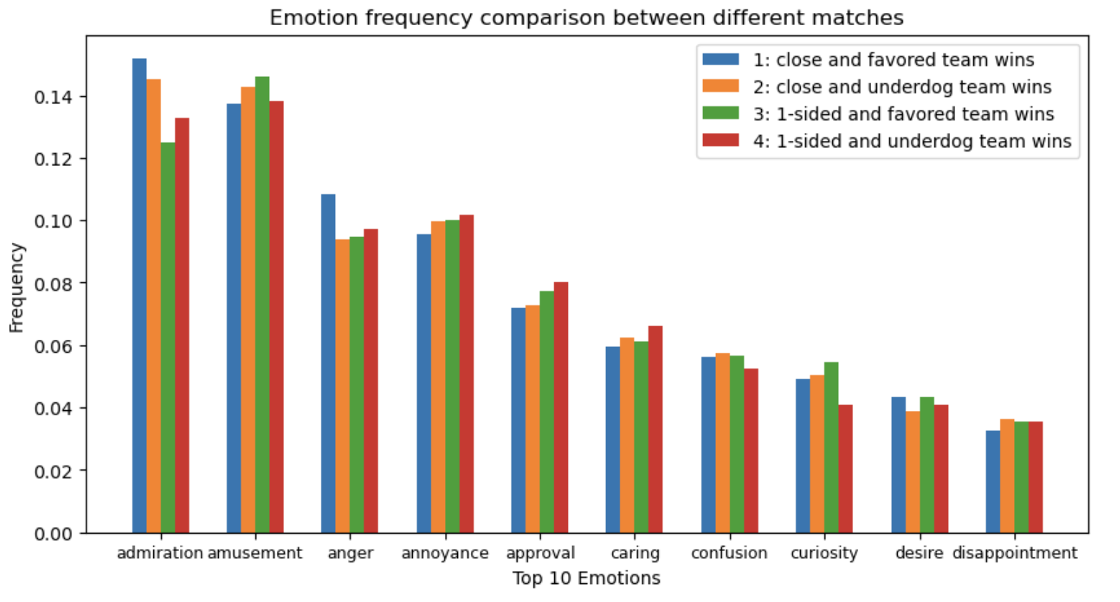
\includegraphics[width=8cm]{MatchesComparision.png}
    \caption{Top 10 emotion frequency comparison between football and soccer}
\end{figure}

In Figure 5, we show the emotion frequency comparison between matches in different categories for the top 10 emotions with the highest frequency. When the match is a close one and the favored team wins, emotions of admiration and anger appear most frequently. When the match is one-sided and the underdog team wins, the comments in the population show more annoyance, approval, and caring.

\begin{figure}[h]
    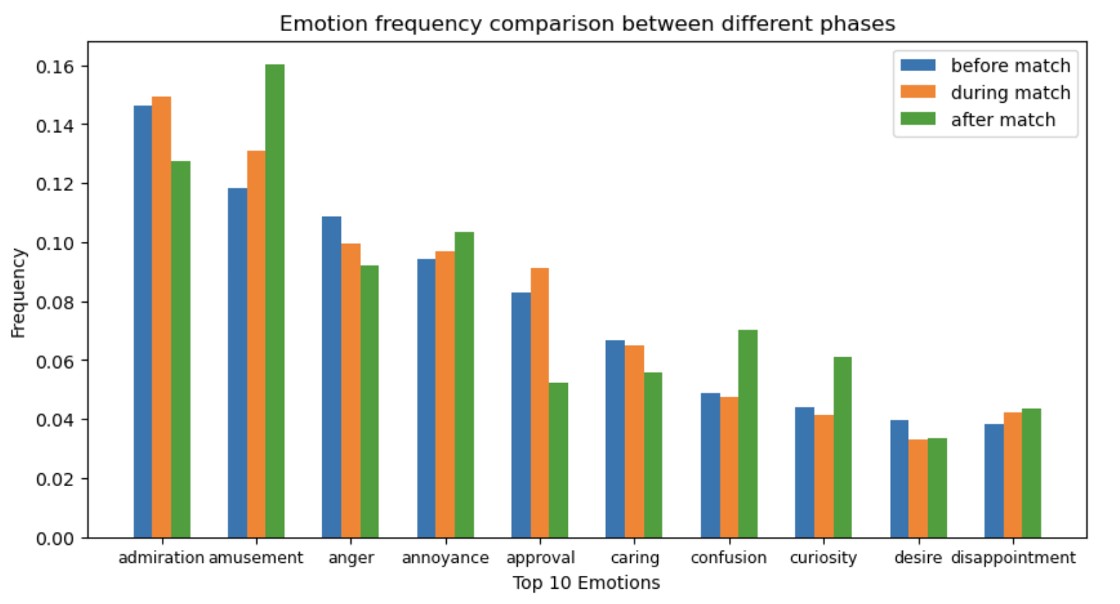
\includegraphics[width=8cm]{PhasesComparision.png}
    \caption{Top 10 emotion frequency comparison between different phases}
\end{figure}

We also show the emotions change in the population when the match is in different phases in Figure 6. We investigate the comments in three phases: before matches, during matches, and after matches. In general, people have more anger and caring before matches than in the other two phases. More admiration and approval are observed during the matches than in the other two phases. And comparing to the other two phases, we see more amusement and annoyance after matches.


\section{Experimentation}

\subsection{Match Outcome/Sport Prediction}
We created a classification model using Decision-Tree, which we settled on after testing with other models and finding it to be the best for predicting category/sport using only phases and emotion-labels(no comment text data used as feature). 

The result when predicting just the 4 victory outcomes(1-sided vs. close; favored team vs. underdog team) gives us an accuracy of around 0.40, but what is interesting about the results is that the F1 score is higher for games in which the favored team won vs. underdog team by around 0.10. When splitting the target into more classes of the emotion coming from neutral, favored, or underdog team fans. We can see that most of the accuracy comes from neutral members, as they are the largest group. However, the most interesting is that the highest precision comes from not the neutral comments but from favored team fans in which the match is 1-sided and the underdog team wins. 

When using the model to predict between the 2 sports(Football vs Soccer), the model does better than random chance with a score of 0.70 accuracy. Some interesting findings from this are that recall is very low for Football at 0.57 but a lot higher for Soccer at 0.82. The F-1 scores for both are 0.65 and 0.74.

\subsection{Reddit Thread Generation}
We sought to use our data to predict how a theoretical game, like an Eagles vs Rams Super Bowl would look like. This would mean training a Sequence to Sequence model that inputs and outputs English. We tried doing this by using two EncoderDecoder models. The encoder for our new model was taken from Google's BERT to BERT English to German transformer model \cite{DBLP:journals/corr/abs-1907-12461}. We give it a context, which contains the game information like the team names, scores, match MVP etc. The encoder performs self-attention on this (tokenized) context to give us the attended tokens. We then use these tokens as the Key and Value in our decoder to perform cross-attention, which is the mirrored version of the encoder model, i.e., German to English. 

During the fine-tuning process, the decoder predicts the next token given a tokenized Reddit comment using the aforementioned cross attention. The loss is the Cross-Entropy loss of the predicted token and the target token.

After the model has finished training, the model is used for generation. We give it a custom context and a starter token(s). We then let the model generate infinitely till it either hits an EOS token or till it hits a predefined generation length.

\section{Conclusion}
The project highlights that there are indeed significant differences between the types of emotions exhibited by the supporters of winning and losing teams based on their winning odds and the manner of victory/loss. These emotions change from the type of loss to the time at which they're captured as well. These findings are significant for researchers, marketing practitioners, and consumers themselves for multiple reasons. 
\section{Contributions}

\textbf{Sameed Khan}: Project idea and conceptualization, data gathering, some pre-processing, report writing, analysis of individual commenters' data, and presentation.

\noindent\textbf{Jianfeng Ke}: Majority of the visualization of the main results.

\noindent\textbf{Sean Lynch}: Majority of data collection and pre-processing, some visualization of results, input in analysis of results.

\noindent\textbf{Anveshak Rathore}: Creating and finetuning the Sequence to Sequence transformer model on our analysed data. 

\noindent\textbf{Daheng Kuang}: Wrote the base code for loading the pre-trained Bert model and also the code for scraping the Reddit API data. Created and tested the Decision-Tree model. 

\bibliographystyle{acl_natbib}
\bibliography{acl2018}

\end{document}
